%%%%%%%%%%%%%%%%%%%%%%%%% DO NOT CHANGE %%%%%%%%%%%%%%%%%%%%%%%%%%%
\documentclass[12pt]{article}
%%%%%%%%%%%%%%%%%%%%% END OF DO NOT CHANGE %%%%%%%%%%%%%%%%%%%%%%%

\usepackage[utf8]{inputenc}
\usepackage{setspace}
\usepackage{cite}
\usepackage{graphicx}
\usepackage{float}

%%%%%%%%%%%%%%%%%%%%%%%%% DO NOT CHANGE %%%%%%%%%%%%%%%%%%%%%%%%%%%

\setlength{\marginparwidth}{0pt}
\setlength{\marginparsep}{0pt} 
\setlength{\evensidemargin}{0.25in}  

\setlength{\oddsidemargin}{0.25in} 
\setlength{\textwidth}{6.375in}

%%%%%%%%%%%%%%%%%%%%% END OF DO NOT CHANGE %%%%%%%%%%%%%%%%%%%%%%%
\title{Research Proposal}





\author{Andy Mai, Md Iztiba, Phu Anh Pham, Bo Wei Yao, TJ LeBlanc}
\date{\today}


%%%%%%%%%%%%%%%%%%%%%%%%% DO NOT CHANGE %%%%%%%%%%%%%%%%%%%%%%%%%%%
\linespread{1.5}
%%%%%%%%%%%%%%%%%%%%% END OF DO NOT CHANGE %%%%%%%%%%%%%%%%%%%%%%%

\begin{document}
\maketitle

\section*{Abstract}
Working from home has become an increasingly popular medium of work due to the onset of COVID-19 and its ramifications. With the pandemic and developments in internet speeds, access to communication software and the need to connect remotely, remote work has become ever more popular. Since the word “telecommuting” was first used in the 1970’s, researchers have studied the effects it has on the worker and company, particularly if it has any merits or detriments. 

Our main objective in this literature review and research is the effects of remote work on workers to better understand its implications. In studying other research that has been done on the subject, we hope to shed a light on remote work and its benefits and drawbacks that have already been conducted. We have also done our own research in order to compare and contrast how the past sentiments and findings may have changed. 

Our review uses key categories we have identified to be particularly important to the implications for employees who work from home, including self leadership, health, time, work-environment, and training and career development. We then state our own research findings and the implications, differences, and issues faced. Finally our synthesis will conclude with key next steps such as things we would change, recommendations for those who do work remotely, how the research could have been improved, and any advice we would give to companies and future researchers. 

\section*{Literature Review}

\subsection*{Self leadership}
Working from home has enabled many people to work flexible hours and gain control of their lives. Many companies have now switched to a “Results Only Work Environment” or ROWE, where employees can work from anywhere and for any amount of time as long as assigned work is completed. This has shown to boost internal motivation due to the working environment being better and employees feeling a sense of self-leadership \cite{Abdul}. Companies have also realized that work from home is here to stay and that they need to adapt to this changing work environment. Thus, companies have started programs targeted at boosting self-leadership and motivation levels for employees not in the office \cite{sultana2021exploring}. Studies have shown the best ways to do this are giving employees autonomy, a sense of power and flexible working hours \cite{sultana2021exploring}. 
 
On the other hand, companies that do not empower their work from home employees have shown to have worse work environments. Managers who make all the decisions have been shown to have worse employee relationships, lower motivation levels and higher employee turnover. In fact, studies have shown that there is a 40.19\% correlation between worker satisfaction and productivity \cite{sultana2021exploring}. Satisfaction was seen to be higher when employees were given more trust by their managers to get the job done and not micromanaged even when working from home, thus leading to higher productivity \cite{sultana2021exploring}.

\subsection*{Health}

As the world comes out of the pandemic, we can learn more about the potential health benefits and negatives of remote work. Aside from the indirect benefits of remote work for mental health and stress from increased control of their time, there are also numerous direct health benefits as well \cite{doi:10.1177/1529100615593273}. Some of these include a significant reduction in work-related stress and exhaustion as a direct result of having that control. There is also evidence to show the lack of travel due to remote work is actually a health benefit as well, as one study has shown that there is a negative correlation between those who commute and physical activity levels of those that do not\cite{HOEHNER2012571}. Another area of consideration has been the potential time saved from commuting and what that time could potentially be used for in terms of improving one's health. Studies have shown that people who do not commute to the office tend to eat less fast food and increase time spent at a gym \cite{allen2008workplace}.

However, there are negative health considerations associated with the prevalence of remote work. The ergonomics of the working space has a major impact on health, which offices have standards and controls for but are not always present for remote work environments. Things to consider include back support, monitor height, arm rests and the location of keyboards and mice which can all contribute to detrimental work from home health and can increase risk of injury\cite{ellison2012ergonomics}. 

\subsection*{Time}

Employees may minimize commute times by at least one and a half hours by remote working, allowing them to leave work early and have more time for their personal life \cite{george2022}. In addition, people experience less stress and are more productive as they can use the time saved from commuting to sleep more and feel better in the morning \cite{george2022}.

Other studies suggest that job satisfaction also increases when remote employment allows employees more autonomy, time to satisfy their job, family, and life \cite{natasha2016}. For instance, people can eat dinner with their families soon after their shift ends instead of spending more than thirty minutes traveling back home and feeling irritated by traffic congestion. Having high-quality time with family is vital to one’s emotions and mental health, and employees do more excellent quality work when they are in a pleasant mood and healthy mentality. Also, research on the effects of remote working during COVID-19 has shown that employees produce higher quality work because they have longer breaks in between and can have flexibility in their shifts \cite{wangb2021}.

Although remote work gives employees more personal time, there are some obstacles when working at home regarding time. Employees may use the time saved from commuting to prepare meals (breakfast, lunch, dinner) for the whole family, which consumes considerable time and decreases their focus on work quality. In addition, employees spend more time assisting children and family members during the work shift and as a result, employees deal with more stress on the family conflict side, and their job productivity may be lower. 

\subsection*{Work environment}

Working in a home environment can provide significant benefits over working in an office. One commonly seen problem with working in an office environment is distractions resulting from needing to constantly interact with co-workers. This is made much worse in offices that are open-plan, where noise and a lack of privacy also become very apparent concerns \cite{Kim2013}. Working from home helps solve these issues since employees would not need to deal with co-workers in person while also not being exposed to the generally chaotic nature of office environments. Employees are also given more flexibility to interact with their families due to not having to spend a large portion of their day away from home, which can contribute to a better work-life balance that improves both mental and physical health \cite{Xiao2021}. Additionally, it is essential for a work environment to have good lighting, ergonomics, air quality, acceptable temperature and humidity, and a low level of noise to ensure that a worker is satisfied and able to work at peak efficiency \cite{Xiao2021}. One of the benefits of working from home is that an employee has full control over these factors since it is their own home. This gives them the ability to customize aspects of their workspace as they wish, which can give them a great deal of satisfaction and comfort in comparison to being confined to a small cubicle \cite{Xiao2021}.

However, it is important to note that these benefits can greatly vary depending on many factors such as socioeconomic groups, occupations and industries that remote workers are in \cite{Etheridge2020}. For instance, in 2020 female workers and low earners generally reported suffering from a loss in productivity when they were forced to switch to remote work \cite{Abi2020}. This was primarily due to their occupations not being compatible with remote work \cite{AbiTasks2020}, and in the case of female workers this includes distractions relating to childcare and other household chores which also played a key role in the reduction of productivity \cite{Chattopadhyay2021}. As a result, these groups were found to have a notable decrease in their mental health due to stress \cite{Etheridge2020}. Stress resulting from social isolation can also become an issue that reduces productivity \cite{Toscano2020}, with this being made much worse for workers who suffer from psychological fragilities \cite{Bouziri2020}. Lastly, musculoskeletal disorders can appear in remote workers if the ergonomics of their workstations are unsatisfactory, resulting in a reduction in both productivity and job satisfaction \cite{Evina2020}.

\subsection*{Training and career development}

Events like COVID-19, followed by mandatory virtual or remote work settings, can have an impact on people's emotional and cognitive reactions, as well as their learning capacities and career development. COVID-19 has undoubtedly altered how human resources professionals and executives prepare people and organizations for change during uncertain times as well as how people react to the change. Emotional control affects how people process information and develop opinions, which can have significant effects on how they prepare for and make decisions about their careers \cite{Restubog2020}. To reduce the negative effects of emotions, one must actively and deliberately look for ways to manage them by participating in emotionally uplifting activities. Constant professional growth through virtual mentoring can also enable peak performance, regardless of one's career level. The chance for communication and professional growth are two benefits of virtual mentoring. It is organizations that will ultimately benefit from employees’ career development \cite{Yarberry2021}.  For more mutually beneficial outcomes, human resource development professionals are tasked to shift development initiatives to a virtual/remote environment in response to the new workplace normal.

Remote employees frequently experience social isolation since they do not have many face-to-face meetings and their communications with coworkers are irregular and limited \cite{Park2021}. They feel removed from decision-making processes and less connected to their organizations \cite{Virick2010}. Furthermore, in the context of distant e-work, the "out of sight, out of mind" approach might weaken the importance of personal connections. This might result in a person's career stagnation and professional growth, as well as limited access to social support systems including informal learning and mentorship \cite{Smith2018}.

Employees who were further along in their careers may have been shielded from the effects of missed opportunities for professional growth. This is demonstrated by the study's findings, which show that just seven percent of those over 55 say they would think about quitting their workplace if they did not receive more training and assistance. Instead, younger employees—a group most likely to gain from participating more fully in peer interactions and picking the brains of more experienced colleagues—have taken the brunt of missed chances. Furthermore, over half (46 percent) of workers under the age of 35 claim to have had less opportunities to interact with and learn from their coworkers during this time \cite{Kairinos2022}.

When it comes to becoming ready for the future of work, the workforce has seen significant advancements. Before COVID-19, technologies that are now progressively transforming into mainstays of the workplace setting were not even on employers' radars. With time, we feel optimistic that training leaders and HR managers will embrace more of these new and emerging technologies in a way that will enable the workforce to pursue individual career objectives and open doors to competitive learning opportunities \cite{Kairinos2022}. Employers will be able to achieve potential advantages as well as keep a healthier, more productive staff by offering mindfulness training and coaching to individuals and teams \cite{Mariana}.

\section*{Experimental Design}

\subsection*{Research Question}
How does remote work affect employee productivity?

\subsection*{Hypotheses}
Null hypothesis: remote work has no effect on employee productivity. \\
Alternative hypothesis: remote work has either a positive or negative effect on employee productivity. 

\subsection*{Variables}
There are a number of variables that we are considering into measuring employee productivity: \\
Major variables:
\begin{itemize}
  \item Self leadership 
  \item Mental health 
  \item Work environment 
  \item Time
\end{itemize} \\
Minor variables:
\begin{itemize}
  \item Training and career development 
  \item Physical health 
  \item Pay
  \item Tooling (communication, work essential tools)
  \item Process and Support (help desk, manager support)
\end{itemize}

\subsection*{Methodology}
We have decided to proceed with a quantitative approach for this experiment. We believe that utilizing data, numbers and graphs, a stronger argument can be provided to back up findings and patterns discovered during the analysis phase of the experiment results. Also, being quantitative provides a more accurate analysis for any patterns or findings, as they can be expressed in precise terms such as numerical differences or percentages.

\subsection*{Data grouping}

That data collected will be grouped and aggregated with a number of demographic information that we collect from candidates. The following variables are considered:

\begin{itemize}
  \item Age group 
  \item Marital status
  \item Kids
  \item Approximate geographical location
  \item Sex
  \item Ethnicity
  \item Career field
\end{itemize}
These will be used for aggregation and grouping during the analysis, discussion and reporting phase. For example, we can use the data to answer questions such as the following:
\begin{itemize}
  \item How does physical health’s impact on employee productivity vary between different age groups?
  \item How does mental health’s impact on employee productivity vary between different races?
\end{itemize}

\subsection*{Data collection}

A questionnaire, created with Google Forms and contains questions with regards to remote work and employee productivity, will be sent out to various websites. \\
All questions will be asked in statements, followed by the following 5 options: 
\begin{itemize}
  \item Strongly disagree
  \item Disagree
  \item Neutral
  \item Agree
  \item Strongly agree
\end{itemize}
The candidate answering the question may only select 1 out of the above 5 options for each question. 

\subsection*{Question scoring}
Values 1 to 5 are assigned on scale between strongly disagree to strongly agree. However, the values are dependent on whether the question is a positive reinforcement to employee productivity. \\
In a positive reinforcement scenario, such as: 
\begin{itemize}
  \item I feel less stressed when I’m working from home. 
  \item I am more productive when I’m working from home. 
\end{itemize}
The option of strongly agree would be assigned a value of 5, while the strongly disagree option would be assigned a value of 1. \\
However, in a negative reinforcement scenario, such as: 
\begin{itemize}
  \item I tend to burn out from working remotely.
  \item I miss face to face contact with colleagues.
\end{itemize}
The vice versa is true. Strongly agree would be assigned a value of 1, while the strongly disagree option would be assigned a value of 5.

\subsection*{Assumptions}
There are several assumptions that we need to make in order to measure employee productivity from this experiment successfully.

\begin{itemize}
  \item Better trained / more qualified for the job = higher productivity
  \item Having better health (mental, physical) = higher productivity
  \item Higher pay = higher productivity
  \item Better tooling = higher productivity
  \item Better support= higher productivity
  \item Negative or disruptive environment = lower productivity
  \item More or complicated processes = lower productivity
\end{itemize}

\subsection*{Questionnaire}
Please see Appendix A for the complete questionnaire.

\section*{Experimental Result}\

\subsection*{Tooling}
The numerical analysis stack from Python is used to conduct analysis on the results we collected from the questionnaire. The stack includes Pandas, which is used in storing and manipulating tabular data, Matplotlib, which is used for graphing, and Jupyter Notebook, which is used for presentation.

\subsection*{Analysis process breakdown}
\begin{enumerate}
  \item Download questionnaire results from the Google forms in csv format
  \item Read csv file in and create a Pandas dataframe from that
  \item Do some data cleaning
  \item Interpret the results into numerical values, according to the rules outlined in the Question Scoring section
  \item Calculate total and mean columns
  \item Perform group by function between different demographics groups
  \item Plot the resultant table in a bar graph and present it
\end{enumerate}

\subsection*{Analysis types}
There are two types of analysis that have been performed: vertical and horizontal analysis. \\
Vertical analysis:

Pick out an independent variable, such as mental health or work environment,  and look at it independently across different demographics groups to see how this particular factor differs.
\begin{figure}[h]
    \centering
    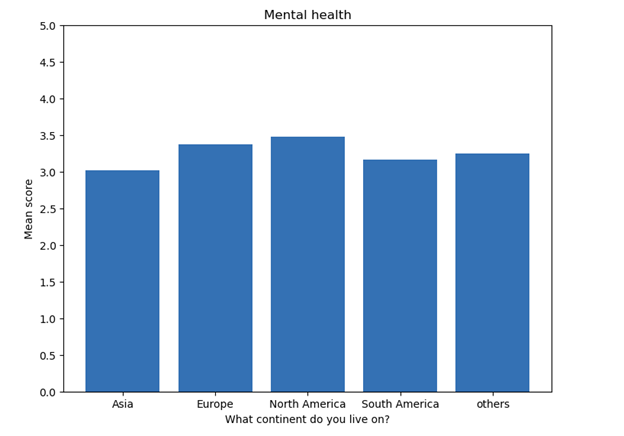
\includegraphics[scale=1]{vertical.png}
    \label{vertical}
\end{figure} \\
Horizontal analysis:

Pick out an individual demographic group, such as sex or career field, and look at the differences between all the factors for that particular group across the board.
\begin{figure}[h]
    \centering
    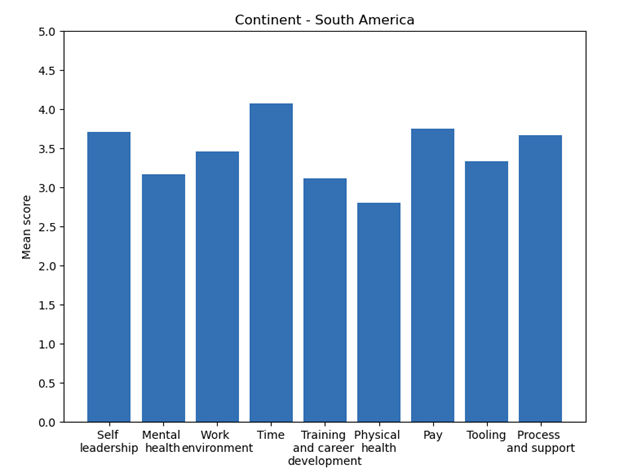
\includegraphics[scale=1]{horizontal.png}
    \label{horizontal}
\end{figure} \\

\section*{Experimental findings}

\subsection*{Unhappy Asia}

Here’s the overall happiness score compare between Asian and Europe.

\begin{figure}[h]
    \centering
    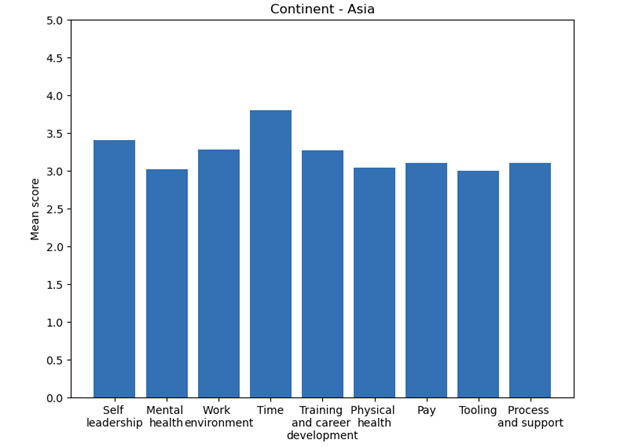
\includegraphics[scale=1]{asia.png}
    \label{asia}
\end{figure} \\

\begin{figure}[h]
    \centering
    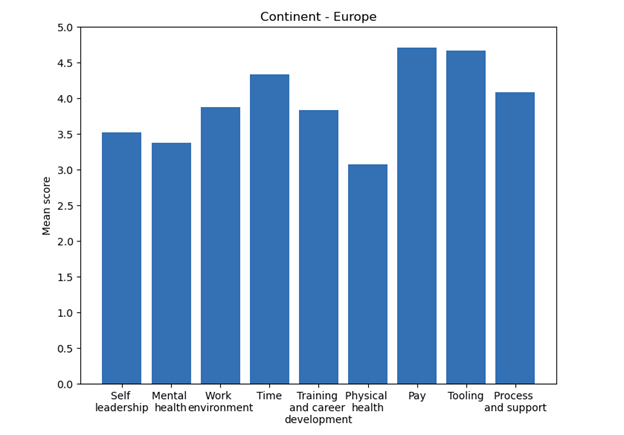
\includegraphics[scale=1]{europe.png}
    \label{europe}
\end{figure} 

People who work in the Asian continent scored slightly lower (difference of $< 1.0$)  in multiple categories, including self leadership, mental health, work environment, time, training and career development, and process and support. Asia scored significantly lower (difference of $\geq 1.0$) in the pay and tooling categories. 

A number of countries with high population density are known for their high intensive work schedules. The rule of 996 is commonly employed across China, which means a work week of 9am to 9pm, Monday to Saturday for six work days a week. South Korea is known for having one of the highest suicide rates due to work stress out of all the developed countries in the world. \cite{suiciderate2022}

The change to remote work did not seem to have changed the work condition by much for people in Asia, as they are overworked, less supported and underpaid.

\subsection*{Kids and marriage}

There’s a slight dip in mental health happiness between people who have kids and people who do not. There’s a bigger dip in mental health between married workers versus single or workers in the “Others” category, which can be assumed to be either divorced or in common law.

\begin{figure}[h]
    \centering
    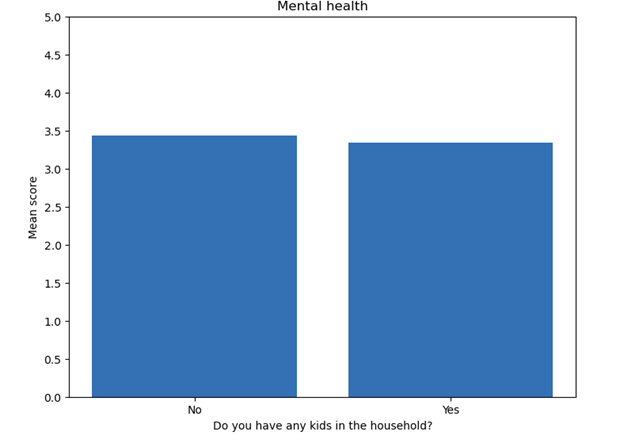
\includegraphics[scale=1]{kids.png}
    \label{kids}
\end{figure} \\

Families with kids find that their mental health is impacted more. One possible cause of this is that kids, especially young ones, tend to serve as a distraction in their work environment, which will potentially lead to a higher level of stress. 

Married workers have the highest score in the mental health category. One can argue that a married worker can find more sense of safety and comfort in their relatively stable relationship status. 

In summary of the above two findings, in order to achieve maximum mental health, the best combination would be to be married but have no kids.

\begin{figure}[H]
    \centering
    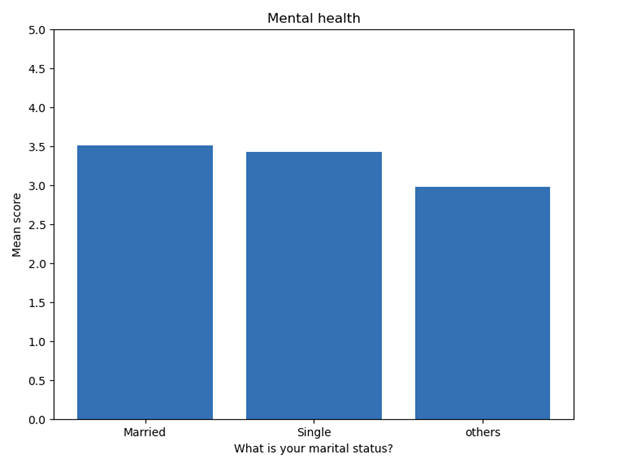
\includegraphics[scale=1]{marriage.png}
    \label{marriage}
\end{figure} 

\subsection*{IT and marketing}

Here are the overall happiness scores of IT and marketing workers across the board.

\begin{figure}[h]
    \centering
    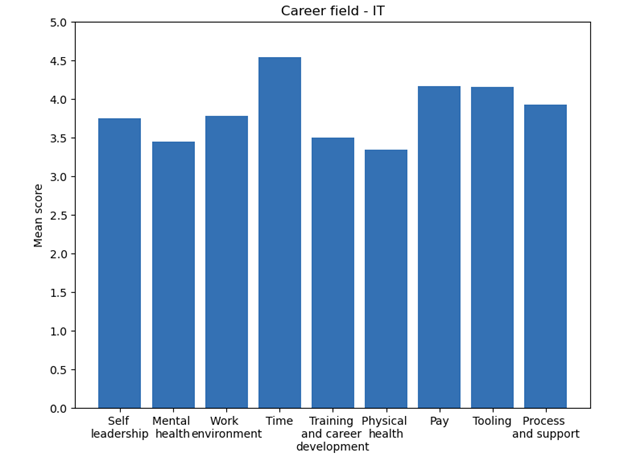
\includegraphics[scale=1]{it.png}
    \label{it}
\end{figure} \\

\begin{figure}[h]
    \centering
    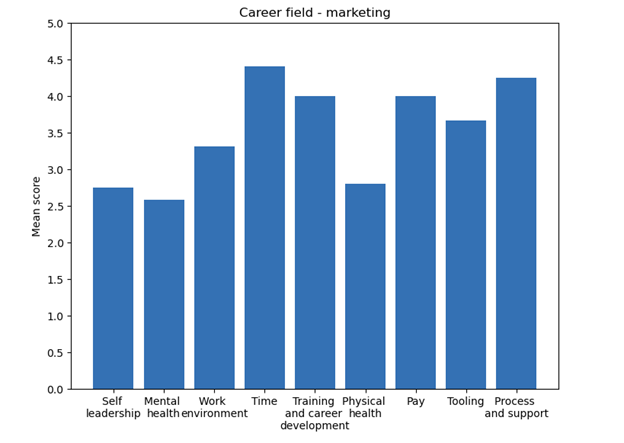
\includegraphics[scale=1]{marketing.png}
    \label{marketing}
\end{figure} 

When doing a side by side comparison between IT and marketing demographics groups, we found a significant drop (around 1.0)  in the self leadership and mental health categories from IT to marketing workers. 

IT workers are capable of working in solitude for hours - chipping away at a problem, working out solutions, coding and testing. For the majority of IT workers, it doesn’t make a sizable difference whether the above tasks are performed from home or at the office. 

However, marketing is all about connecting with customers and resonating with customers with the right product, price and value. The people who work in marketing have a need to establish and feel that close connection with people on a daily basis during their work routine. Therefore, when someone in marketing is forced to work in isolation at home for prolonged periods, they tend to lose the motivation and self leadership needed to perform work efficiently. The marketing workers also suffer in the mental health category due to reduced time for face to face connection with others. 

\subsection*{The 46-55s group}

See the following graphs for the mental health variable across different age groups, overall scores across the board for age group 26-35, and age group 46-55.

\begin{figure}[h]
    \centering
    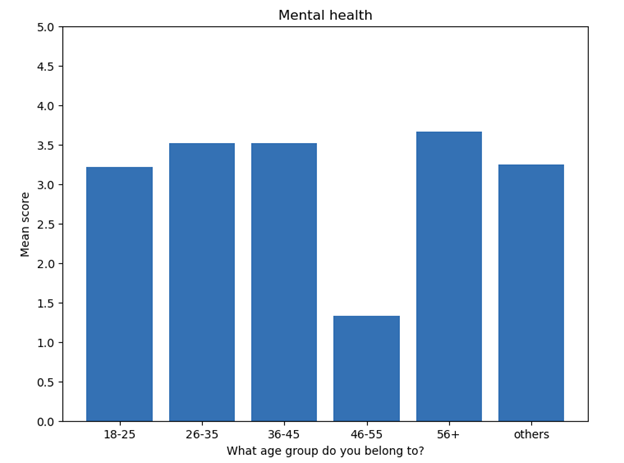
\includegraphics[scale=1]{mental.png}
    \label{mental}
\end{figure} \\

\begin{figure}[h]
    \centering
    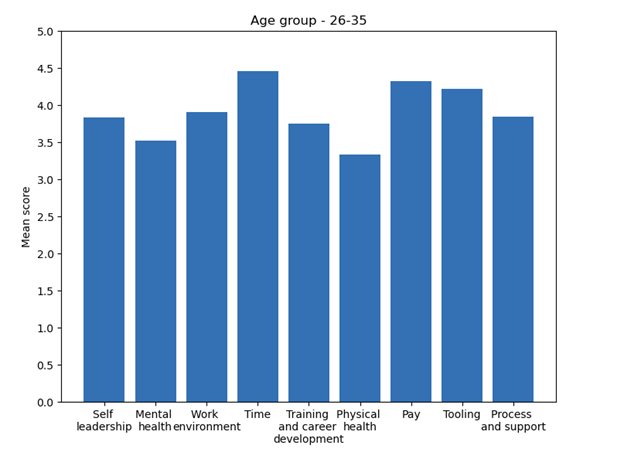
\includegraphics[scale=1]{26.png}
    \label{26}
\end{figure} \\

\begin{figure}[h]
    \centering
    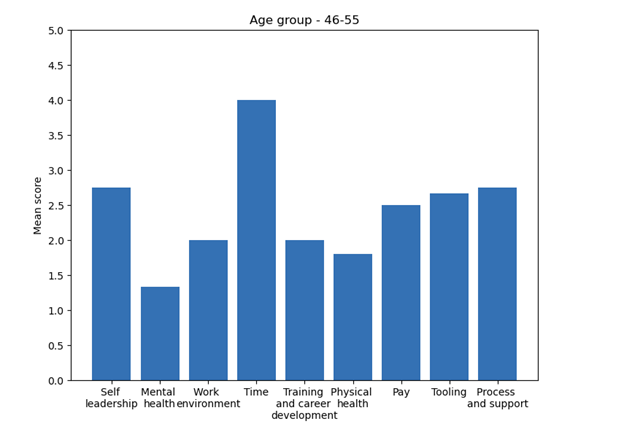
\includegraphics[scale=1]{46.png}
    \label{46}
\end{figure} 

There is a significant drop all across the board for the age group 46-55, particularly severe in mental health, work environment, physical health, and training and career development.

The age group 46-55 falls into the demographics category of Generation X, which is also known as the worst generation. These people would have started work somewhere between late 80s to early 90s. For the past twenty to thirty years, Generation X’s days have been building on the same routine, day in day out. Therefore, this remote work change does not come easy to them.

Generation X are not known to be avid adopters of technology. They prefer phone calls if remote, however face to face still remains as their premier choice of communication. Many of the workers in the age group 46-55 have only learned the minimum amount of technology required in order to stay relevant in their job field.

The second factor is that the people in the age group 46-55 may currently be experiencing their midlife crisis. A good number of them are married with kids, and this is the time to pay for their post secondary tuition. Many of them are burdened with healthcare bills for their ailing parents. These are all potential stress factors in their lives, not counting the personal problems that they are currently dealing with at the moment. 

Lastly, those in Generation X still have a number of years to go before retirement. Perhaps some of them are unhappy with where they are currently in the career ladder, despite only having a limited number of years left in their respective job field. 
All the factors above combined and aggregated into this result that we are seeing in this experiment. 

\section*{Bias}

A number of biases exist in this experiment. The questionnaires are sent out on open forums, therefore anyone with access to the Internet has access to them and has the power to fill it out. This may invite auto survey filling bots, or speedrunners whose aims are to finish as many surveys as possible within a specific time frame instead of taking the time to provide accurate and truthful data.

We also see a number of biases based on the results we have collected: \\
This experiment is heavily biased towards IT and customer service workers.
\begin{figure}[h]
    \centering
    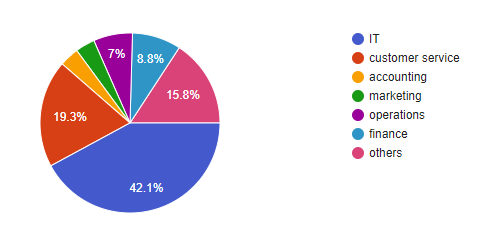
\includegraphics[scale=1]{bias_it.png}
    \label{bias_it}
\end{figure} 

This experiment has zero African candidates for representation as of the time we are conducting this analysis. 
\begin{figure}[h]
    \centering
    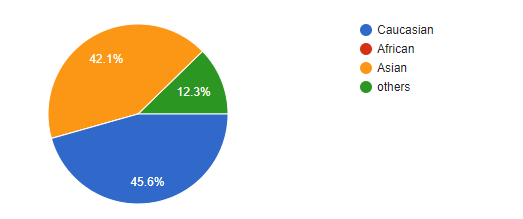
\includegraphics[scale=1]{bias_race.png}
    \label{bias_race}
\end{figure} 

This experiment is heavily biased towards North American continent residents.
\begin{figure}[H]
    \centering
    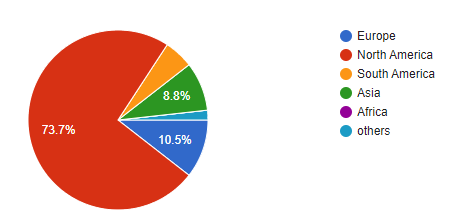
\includegraphics[scale=1]{bias_na.png}
    \label{bias_na}
\end{figure} 

This experiment is geared towards more single workers than others.
\begin{figure}[h]
    \centering
    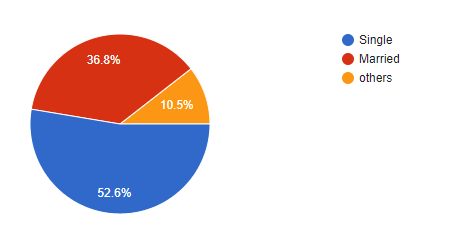
\includegraphics[scale=1]{bias_marriage.png}
    \label{bias_marriage}
\end{figure} 

The majority of correspondence have no kids in the household.
\begin{figure}[h]
    \centering
    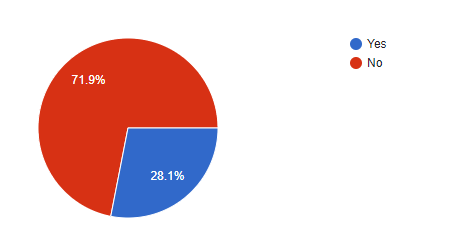
\includegraphics[scale=1]{bias_kids.png}
    \label{bias_kids}
\end{figure} 

\section*{Discussion}
\subsection*{Summary of findings from literature review}

From the self-leadership and health perspective, working from home increases worker satisfaction and productivity because of the working environment and the sense of self-leadership are achieved. Health is also improved as employees eat out less and spend more time in the gym. However, there are negative health impacts such as respiratory inflammation or back injury if the home working environment does not meet the minimum requirement.

Employees have greatly benefited from having a better work-life balance and productivity in terms of time and the work environment. They saved time going to work and had those extra hours to spend with friends and family or on themselves. Employees may personalize their working environment to make it more comfortable for them. Whether working from home or on-site, there have been instances where employees have lost focus owing to various distractions, causing the quality of their work to suffer.
 
Employees suffered greatly from social isolation in terms of training and career development, limiting their opportunities for advancement. During the COVID-19 pandemic, employers implemented critical training approaches and virtual mentorship to prevent productivity drops and employee turnover.

\subsection*{Summary of findings from experiment}

\begin{itemize}
  \item Asia has a lower overall happiness score in comparison to Europe. The scores dip significantly ($\geq 1.0$) in the pay and tooling categories, while dipping slightly ($< 1.0$) in self leadership, mental health, work environment, time, training and career development, and process and support. 
  \item In order to maximize mental health for workers, it’s best to be married but have no kids.
  \item Marketing workers suffer in the self leadership and mental health categories after the transition to remote work. IT workers remain relatively unfazed after the transition.
  \item The workers in the 46-55 age group experience a significant drop ($> 1.5$) in score in nearly all categories in comparison to the 36-35 age group.
  \item This experiment is heavily biased towards IT and customer service workers, non African candidates, people who reside in the North American continent, and workers with no kids.
\end{itemize}

\subsection*{Comparison between findings}

The results of both the literature review and the experiment were relatively similar. For instance, the negative impact that having kids can have on a remote worker in terms of distractions and stress was made evident in both the literature review and the experiment itself. Both the literature review and the experiment also indicated that the overall experience of working from home can differ depending on occupations and location. In the case of the experiment, this was seen by the fact that remote workers from Asia had a lower happiness score in comparison to those from Europe, and that marketing workers seemed to suffer much more than IT workers when they had to transition to remote work. For the latter, social isolation seemed to be one of the primary factors as to why marketing workers had a worse remote working experience, which was a factor brought up by the literature reviews done on work environment and training and career development. Overall, the results for both the literature review and experiment seemed to point towards a conclusion that is neither “yes” or “no” in regards to whether or not remote work is good or bad. The effect that remote work can have on people is mostly dependent on many different factors that can greatly differentiate from person to person.

\section*{Future work}

Our results have shown that people saw an increase in productivity and happiness when working from home overall, but were heavily dependent on the field that workers were in. We believe that the logical next steps would be to control for different fields of work when conducting surveys, to compare different fields of work in relationship to the happiness level of the workers. We also saw that there is a significant variance comparing regional happiness levels, which should also be controlled should we or another group conduct another study in this field, they should control for regional differences or study the regional happiness levels.

We would also include ways to limit biases and have a much broader data size in any future work. Our sample size was limited by our budget, time, and available mediums for conducting data gathering. Because of this, biases may have been introduced by factors such as language, field of work, location, and age. Future research would need to address these issues and select a larger data size than the one we had in order to get more accurate and inclusive results while also working to limit biases in the data. 

Based on our research, we have also seen that employee happiness seems to heavily correlate to productivity and employee retention. Thus, the natural future question then arises about how to control and improve employee happiness to maximize productivity. Another question would be to study the causation of happiness and the other variables, such as if happiness causes increased productivity or if some people believe their productivity leads to better happiness. We believe these to be promising paths for future research. It is suggested that company decision makers also study these factors to improve employee retention and worker satisfaction.

\section*{Conclusion}

Overall it can be seen that working from home has had a positive impact on worker happiness and health, while having no downsides to productivity. However results were heavily dependent on the field that people worked in and the amount of autonomy they were given. People tended to live healthier lives from eating out less and cooking more and the time saved commuting was used on working out or sleeping more. Through our literature review, we were able to see that while there were downsides to working from home such as potential stress from family and bad ergonomics, the majority of people had a positive experience with the switch. At the same time, people tended to have a lower sense of community with those in their offices and could experience social isolation. 

We originally wanted to study the effects of working from home in order to see if working from home had any impacts, and through the research we conducted, we saw the same trends as our literature review. The questions we had going in were answered, although with a smaller sample size than we would have liked. We demonstrated that young people found themselves much more happy while those who are older tended to see less benefit. At the same time, productivity was overall similar or improved from working from home, meaning the change in work location did not impact employees ability to get the job done. Although dependent on many variables, we successfully demonstrated that people were overall more happy and productive working from home. Thus, company decision makers should consider implementing more work from home jobs in order to boost worker satisfaction and increase productivity.

\bibliography{research_proposal}
%%%%%%%%%%%%%%%%%%%%%%%%% DO NOT CHANGE %%%%%%%%%%%%%%%%%%%%%%%%%%%

\bibliographystyle{ieeetr}
%%%%%%%%%%%%%%%%%%%%% END OF DO NOT CHANGE %%%%%%%%%%%%%%%%%%%%%%%

\appendix
\section*{Appendix A: Experiment questionnaire}

\subsection*{Example question}
I feel that working remotely has saved me time from commuting, allowing me to be more prepared for work in the morning. 
\begin{itemize}
  \item Strongly disagree
  \item Somewhat disagree
  \item Neutral
  \item Somewhat agree
  \item Strongly agree
\end{itemize}
All categorical questions will have the above answering format.
\subsection*{Categorical question}
\subsection*{Self leadership}

I have a hard time motivating myself when working remotely. \\
I feel that my creativity is reduced when not interacting with people. \\
I feel less engaged at work when working remotely. \\
I am my own leader when I’m working from home. \\
I’m in control of my schedule and pace when I'm working from home. \\
I’m capable of spending less hours accomplishing the same work as before. \\
I am more productive when I’m working from home.  \\
My job allows me to make my own decisions about how to schedule my work.

\subsection*{Mental health}

I feel less stressed when I’m working from home. \\
I feel more socially isolated when I’m working from home. \\
I crave interactions with real people when I’m working from home. \\
I have a hard time separating work from personal life. \\
I feel like I'm at work all the time.  \\
I tend to burn out from working remotely. \\
I feel isolated despite the usage of digital technologies for communication. \\
I miss face to face contact with colleagues. \\
I feel exhausted when working from home. \\
I suffer from anxiety or depression after spending prolonged periods at home. \\
I feel lonely when working from home. \\
I have increased conflicts with family members when working from home. 

\subsection*{Work environment}

I enjoy having the flexibility of working from home.  \\
I have a better work-life balance because of working from home. \\
My family (partner, kids, parents) often interfere with my work routine when I’m WFH. \\
I’m frequently distracted when working from home.  \\
Having remote work has given me plenty of room to focus on deliverable items.  \\
I am more organized when I’m working from home.  \\
I experience family work conflict when working from home. \\
I am able to create an isolated space for work at home.

\subsection*{Time} 

I feel that working remotely has saved me time from not having to commute. \\
I feel that working remotely has saved me time from not having to get up early. \\
I feel that working remotely has saved me time from not having to get home late. \\
I’m able to work on chores during downtimes at work.  \\
I have more time meeting with friends or going to the gym.

\subsection*{Training and career development}

I feel that remote work has reduced my chance of being promoted. \\
I feel that my company is offering less training programs because of remote work. \\
I am capable of working on personal development and growth when working remotely.


\subsection*{Physical health}

I feel that my physical condition has decreased as a result of not going out to work everyday.  \\
I have more time to spend on physical activities as a result of remote work. \\
My diet improves when I’m working from home.  \\
I spend less time grooming myself when I’m working from home.
My workspace is ergonomic. 

\subsection*{Pay}

My company has cut my pay as a result of remote work. \\
I’m forced to transition to part time as a result of remote work. \\
I believe my raise was reduced as a result of remote work. \\
I believe my bonus was cut as a result of remote work. 

\subsection*{Tooling} 

I had a difficult time arranging together my work station for remote work.  \\
I had a difficult time installing appropriate communication tools for my remote work.  \\
The tools  provided were good enough for my work purposes. 

\subsection*{Process and Support}

I received plenty of support from my supervisor during my remote work. \\
I received plenty of support from my coworkers during my remote work. \\
The IT support was easy to reach during my remote work. \\
The IT support was able to solve my problems during my remote work.


\subsection*{Candidate demographics questions}

What age group do you belong to? \\
18-25, 26-35, 36-45, 46-55, 56+, others \\ \\
What is your marital status? \\
Single, married, others \\ \\
Do you have any kids in the household? \\
Yes, no \\ \\
What continent do you live on? \\
Europe, North America, South America, Asian, Africa, others \\ \\
What is your sex? \\
M, F, others \\ \\
What do you identify as? \\
Caucasian, African, Asian, others \\ \\
What is your career field? \\
IT, customer service, accounting, marketing, operations, finance, others 


\end{document}
